\documentclass[12pt]{article}
\usepackage[margin=2.5cm]{geometry}
\usepackage{enumerate}
\usepackage{amsfonts}
\usepackage{amsmath}
\usepackage{fancyhdr}
\usepackage{amsmath}
\usepackage{amssymb}
\usepackage{amsthm}
\usepackage{mdframed}
\usepackage{graphicx}
\usepackage{subcaption}
\usepackage{adjustbox}
\usepackage{listings}
\usepackage{xcolor}
\usepackage{booktabs}
\usepackage[utf]{kotex}
\usepackage{hyperref}

\definecolor{codegreen}{rgb}{0,0.6,0}
\definecolor{codegray}{rgb}{0.5,0.5,0.5}
\definecolor{codepurple}{rgb}{0.58,0,0.82}
\definecolor{backcolour}{rgb}{0.95,0.95,0.92}

\lstdefinestyle{mystyle}{
    backgroundcolor=\color{backcolour},
    commentstyle=\color{codegreen},
    keywordstyle=\color{magenta},
    numberstyle=\tiny\color{codegray},
    stringstyle=\color{codepurple},
    basicstyle=\ttfamily\footnotesize,
    breakatwhitespace=false,
    breaklines=true,
    captionpos=b,
    keepspaces=true,
    numbers=left,
    numbersep=5pt,
    showspaces=false,
    showstringspaces=false,
    showtabs=false,
    tabsize=1
}

\lstset{style=mystyle}

\pagestyle{fancy}
\renewcommand{\headrulewidth}{0.4pt}
\lhead{CSC 369}
\rhead{Worksheet 4 Solution}

\begin{document}
\title{CSC 369 Worksheet 4 Solution}
\maketitle

\bigskip

\begin{enumerate}[1.]
    \item

    The following assumptions are made before calculation:

    \begin{itemize}
        \item Each job runs for the same amount of time
        \item All jobs arrive at the same time
        \item Once started, each job runs to completion
        \item All jobs only use the CPU (i.e they perform no I/O)
        \item The run-time of each job is known
    \end{itemize}

    \bigskip

    First, I need to calculate the turnaround time when running three job of length 200
    with the SJF and FIFO schedulers.

    \bigskip

    I will do so in parts.

    \bigskip

    \begin{itemize}
        \item \textbf{Part 1:} Calculating turnaround time with FIFO schedulers

        \begin{align}
            \frac{200 + 400 + 600}{3} = 400
        \end{align}

        seconds.

        \item \textbf{Part 2:} Calculating turnaround time with SJF schedulers

        \begin{align}
            \frac{200 + 400 + 600}{3} = 400
        \end{align}

        seconds.
    \end{itemize}

    Second, I need to calculate the response time when running three job of length 200
    with the SJF and FIFO schedulers.

    \bigskip

    I will do so in parts.

    \begin{itemize}
        \item \textbf{Part 1:} Calculating response time with FIFO schedulers

        \begin{align}
            \frac{0 + 200 + 400}{3} = 200
        \end{align}

        seconds.

        \item \textbf{Part 2:} Calculating response time with SJF schedulers

        \begin{align}
            \frac{0 + 200 + 400}{3} = 200
        \end{align}

        seconds.
    \end{itemize}

    \underline{\textbf{Notes}}

    \begin{itemize}
        \item \textbf{Scheduling:}

        \begin{itemize}
            \item Is a process at which allows one process to use the CPU while
            another is on hold, to make full use of CPU
        \end{itemize}

        \item \textbf{Turnaround Time:}
        \begin{itemize}
            \item Is a performance metric
            \item Is amount of time to execute a particular process $^{[1]}$
        \end{itemize}

        \bigskip

        \begin{align}
            T_{turnaround} = T_{completion} - T_{arrival}
        \end{align}

        \begin{itemize}
            \item $T_{completion}$ $\to$ Time at which the job completes
            \item $T_{arrival}$ $\to$ Time at which the job arrived in the system
        \end{itemize}

        \item \textbf{FIFO scheduling algorithm:}

        \begin{itemize}
            \item Is the most basic scheduling algorithm
        \end{itemize}

        \bigskip

        \underline{\textbf{Example}}

        \begin{center}
        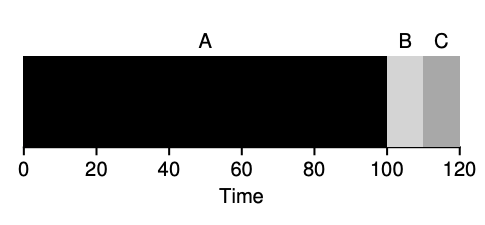
\includegraphics[width=0.6\linewidth]{images/worksheet_4_solution_2.png}
        \end{center}

        \bigskip

        Here, the average turnaround time is:

        \begin{align}
            \frac{100 + 110 + 120}{3} = 110
        \end{align}

        \item \textbf{SJF scheduling algorithm:}

        \begin{itemize}
            \item Is a schduling policy where the shortest job is run first, then the next shortest and so on.
        \end{itemize}

        \bigskip

        \underline{\textbf{Example}}

        \begin{center}
        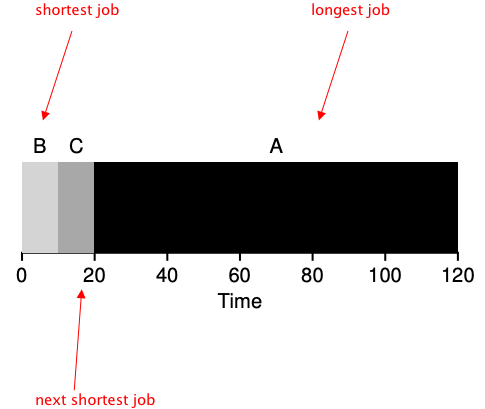
\includegraphics[width=0.6\linewidth]{images/worksheet_4_solution_1.png}
        \end{center}

        \bigskip

        Here, the average turnaround time is:

        \begin{align}
            \frac{10 + 20 + 120}{3} = 50
        \end{align}


        \item \textbf{Response Time:}

        \begin{itemize}
            \item Is amount of time from when a request was submitted until the first response is produced $^{[1]}$
        \end{itemize}

        \begin{align}
            T_{response} = T_{firstrun} - T_{arrival}
        \end{align}

        \begin{itemize}
            \item $T_{firstrun}$ $\to$ First time a job is scheduled
            \item $T_{arrival}$ $\to$ Time at which the job arrived in the system
        \end{itemize}

        \bigskip

        \underline{\textbf{Example}}

        \begin{center}
        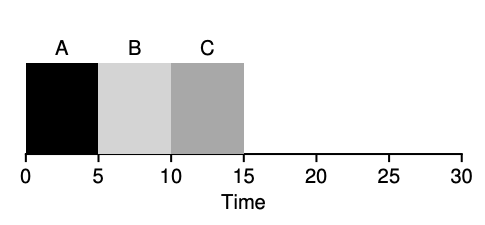
\includegraphics[width=0.6\linewidth]{images/worksheet_4_solution_3.png}
        \end{center}

        \bigskip

        Here, the average response time is

        \begin{align}
            \frac{0 + 5 + 10}{3} = 5
        \end{align}

    \end{itemize}

    \bigskip

    \underline{\textbf{References}}

    \begin{enumerate}[1)]
        \item Old Dominion University, CPU Scheduling \href{https://www.cs.odu.edu/~price/cs471/public_html/spring17/lectures/Scheduling.htm#:~:text=Response%20time%20%E2%80%93%20amount%20of%20time,the%20first%20response%20is%20produced.&text=Associate%20with%20each%20process%20the%20length%20of%20its%20next%20CPU%20burst.&text=Each%20process%20gets%20a%20small,%2C%20usually%2010%2D100%20milliseconds.}{link}
    \end{enumerate}

    \item

    First, I need to calculate turnaround time when running three jobs of different lengths
    $100, 200, 300$ with FIFO and SJF schedulers.

    \bigskip

    I will do so in parts.

    \begin{itemize}
        \item \textbf{Part 1:} Calculating turnaround time with FIFO schedulers

        \begin{align}
            \frac{100 + 300 + 600}{3} \approx 333.33
        \end{align}

        seconds.

        \item \textbf{Part 2:} Calculating turnaround time with SJF schedulers

        \begin{align}
            \frac{100 + 300 + 600}{3} \approx 333.33
        \end{align}

        seconds.
    \end{itemize}

    \bigskip

    Second, I need to calculate response time when running three jobs of different lengths
    $100, 200, 300$ with FIFO and SJF schedulers.

    \bigskip

    I will do so in parts.

    \bigskip

    \begin{itemize}
        \item \textbf{Part 1:} Calculating turnaround time with FIFO schedulers

        \bigskip

        \begin{align}
            \frac{0 + 100 + 300}{3} \approx 133.33
        \end{align}

        \item \textbf{Part 2:} Calculating turnaround time with SJF schedulers

        \begin{align}
            \frac{0 + 100 + 300}{3} \approx 133.33
        \end{align}

    \end{itemize}

    \item
    \setcounter{equation}{0}
    Let the time slice of round robin be 1.

    \bigskip

    First, I need to calculate turnaround time when running three jobs of different lengths
    $100, 200, 300$ with Round Robin schedulers.

    \bigskip

    The answer is

    \begin{align}
        \frac{298 + 499 + 600}{3} \approx 465.67
    \end{align}

    Given that the time of completetion are

    \begin{align}
        &\text{\# of jobs} \times (\text{Len. job 1} - 1) + 1\\
        &= 3 \times (100 - 1) + 1\\
        &= 298
    \end{align}

    for job 1,

    \begin{align}
        &\text{\# of jobs} \times (\text{Len. job 1} - 1) + 2 + (2 \times (\text{Len. job 2} - \text{Len. job 1}))\\
        &= 3 \cdot (100 - 1) + 2 + (2 \times (200 - 100))\\
        &= 299 + 200\\
        &= 499
    \end{align}

    for job 2, and 600 for job 3.

    \bigskip

    Second, I need to calculate response time when running three jobs of different lengths
    $100, 200, 300$ with Round Robin schedulers.

    \bigskip

    The answer is


    \begin{align}
        \frac{0 + 1 + 2}{3} = 1
    \end{align}

    seconds.

    \bigskip

    \underline{\textbf{Notes}}

    \begin{itemize}
        \item \textbf{Round Robin:}

        \begin{itemize}
            \item Solves the problem of having to wait for $x$ number of seconds (e.g 10 seconds)
            before the next job.
            \item Is sometimes-called \textbf{time-slicing}
            \item Does so by running a job for \textbf{time slice} (sometimes called \textbf{scheduling quantum})


            \begin{center}
            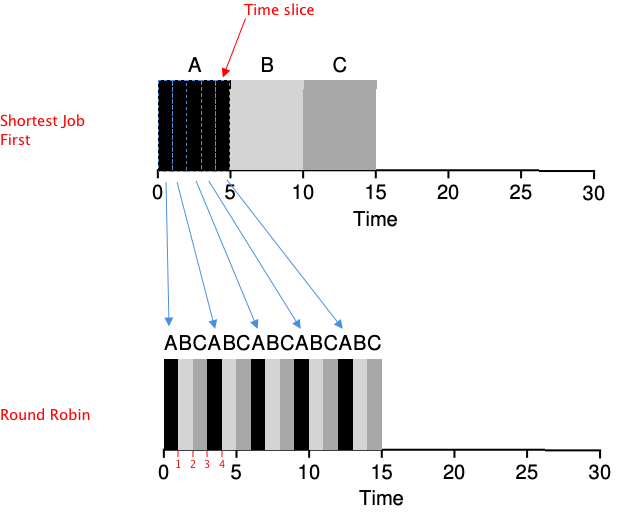
\includegraphics[width=0.8\linewidth]{images/worksheet_4_solution_4.png}
            \end{center}

            \bigskip

            \underline{\textbf{Notes}}

            \bigskip

            In above example, the Response time of Round Robin is

            \begin{align}
                \frac{0 + 1 + 2}{3} = 1
            \end{align}

            seconds.
        \end{itemize}
    \end{itemize}

    \item

    I need to ansewr the types of workloads SJF deliver the same turnaround time as FIFO.

    \bigskip

    SJF delivers the same turnaround time as FIFO when workloads are either

    \begin{enumerate}[1.]
        \item In increasing order by job length (e.g. job 1 has length 100, job 2 has length 200, and job 3 has length 300)
        \item Have the same job length (e.g All jobs have length of 200)
    \end{enumerate}

    \item

    I need to answer answer what types of workloads and quantum lengths does SJF deliver the same response
    time as RR?

    \bigskip

    SJF delivers the same response time as RR when the length of each job is the same
    as the quantum length of each job.

    \item

    As job lengths increase, the average response time also increases.

    \bigskip

    The following simulations are done to demonstrate the relationship between
    job lengths and average response time

    \begin{itemize}
        \item ./scheduler.py -p SJF -j 3 -l 100,100,100 -c
        \item ./scheduler.py -p SJF -j 3 -l 200,200,200 -c
        \item ./scheduler.py -p SJF -j 3 -l 300,300,300 -c
        \item ./scheduler.py -p SJF -j 3 -l 400,400,400 -c
    \end{itemize}



\end{enumerate}

\end{document}